\documentclass[11pt]{article}

\usepackage[a4paper]{geometry}
\geometry{left=2.0cm,right=2.0cm,top=2.5cm,bottom=2.5cm}

\usepackage{ctex} % 支持中文的LaTeX宏包
\usepackage{amsmath,amsfonts,graphicx,subfigure,amssymb,bm,amsthm,mathrsfs,mathtools,breqn} % 数学公式和符号的宏包集合
\usepackage{algorithm,algorithmicx} % 算法和伪代码的宏包
\usepackage[noend]{algpseudocode} % 算法和伪代码的宏包
\usepackage{fancyhdr} % 自定义页眉页脚的宏包
\usepackage[framemethod=TikZ]{mdframed} % 创建带边框的框架的宏包
\usepackage{fontspec} % 字体设置的宏包
\usepackage{adjustbox} % 调整盒子大小的宏包
\usepackage{fontsize} % 设置字体大小的宏包
\usepackage{tikz,xcolor} % 绘制图形和使用颜色的宏包
\usepackage{multicol} % 多栏排版的宏包
\usepackage{multirow} % 表格中合并单元格的宏包
\usepackage{pdfpages} % 插入PDF文件的宏包
\RequirePackage{listings} % 在文档中插入源代码的宏包
\RequirePackage{xcolor} % 定义和使用颜色的宏包
\usepackage{wrapfig} % 文字绕排图片的宏包
\usepackage{bigstrut,multirow,rotating} % 支持在表格中使用特殊命令的宏包
\usepackage{booktabs} % 创建美观的表格的宏包
\usepackage{circuitikz} % 绘制电路图的宏包
\usepackage{cancel}
\ctikzset{logic ports=ieee}     %所有逻辑门使用IEEE标准
\usetikzlibrary{calc}           %使用TikZ中的计算功能

\definecolor{dkgreen}{rgb}{0,0.6,0}
\definecolor{gray}{rgb}{0.5,0.5,0.5}
\definecolor{mauve}{rgb}{0.58,0,0.82}
\lstset{
  frame=tb,
  aboveskip=3mm,
  belowskip=3mm,
  showstringspaces=false,
  columns=flexible,
  framerule=1pt,
  rulecolor=\color{gray!35},
  backgroundcolor=\color{gray!5},
  basicstyle={\small\ttfamily},
  numbers=none,
  numberstyle=\tiny\color{gray},
  keywordstyle=\color{blue},
  commentstyle=\color{dkgreen},
  stringstyle=\color{mauve},
  breaklines=true,
  breakatwhitespace=true,
  tabsize=3,
}

% 轻松引用, 可以用\cref{}指令直接引用, 自动加前缀. 
% 例: 图片label为fig:1
% \cref{fig:1} => Figure.1
% \ref{fig:1}  => 1
\usepackage[capitalize]{cleveref}
% \crefname{section}{Sec.}{Secs.}
\Crefname{section}{Section}{Sections}
\Crefname{table}{Table}{Tables}
\crefname{table}{Table.}{Tabs.}

\setmainfont{Palatino_Linotype}[
  Path = ../Fonts/,
  Extension = .ttf
]
\setCJKmainfont{SimHei}[
  Path = ../Fonts/,
  Extension = .ttf
]
\punctstyle{kaiming}
% 偏好的几个字体, 可以根据需要自行加入字体ttf文件并调用

\renewcommand{\emph}[1]{\begin{kaishu}#1\end{kaishu}}

%改这里可以修改实验报告表头的信息
\newcommand{\studentNum}{00000000}
\newcommand{\name}{我是谁}
\newcommand{\exDate}{2025.03.11}
\newcommand{\weekDay}{二}
\newcommand{\ap}{下午}
%%%%%%%%%%%%%%%%%%%%%%%%%%%

\begin{document}

%若需在页眉部分加入内容, 可以在这里输入
% \pagestyle{fancy}
% \lhead{\kaishu 测试}
% \chead{}
% \rhead{}

\begin{center}
    \LARGE \bf 《\, 基\, 础\, 物\, 理\, 实\, 验\, 》\, 实\, 验\, 报\, 告
\end{center}

\begin{center}
    \emph{学号}\underline{\makebox[6em][c]{\studentNum}}
    \emph{姓名}\underline{\makebox[6em][c]{\name}} 
    \emph{实验日期} \underline{\makebox[8em][c]{\exDate}}
    \emph{星期} \underline{\makebox[2em][c]{\weekDay}}\;\underline{\makebox[3em][c]{\ap}}
    {\noindent}
    \rule[8pt]{17cm}{0.2em}
\end{center}

\begin{center}
    \Large \bf 线性与非线性元件伏安特性的测量
\end{center}

\section*{一、实验目的}

\begin{enumerate}
    \item 熟练使用电学实验的常用仪器,掌握电流、电压、电阻等电学量的测量方法。
    \item 理解制流电路和分压电路的工作原理,学习恒压源与恒流源的使用。
    \item 测量小灯泡的伏安特性曲线,掌握电流表的内接法和外接法。
    \item 测量发光二极管,稳压二极管的伏安特性曲线。
\end{enumerate}

\section*{二、实验原理}

\begin{enumerate}

    \item 制流电路、分压电路、电流表内接法、电流表外接法

    \begin{circuitikz}[european]
        % 绘制电源
        \draw (0,2) to[battery, l=$E$] (4,2); % 电源符号

        % 绘制滑动变阻器(三端连接)
        \draw (0,2) -- (0,0)
            to[pR, name=pot, mirror, european] (4,0) % 水平放置滑动变阻器
            -- (4,2);

        % 添加滑动触点引出端
        \draw (pot.wiper) -- ++(0.7,0) 
            to[short, -o] ++(0,0) node[right] {$U_o$}; % 输出电压标注

        \draw (4,0) -- (4, -0.555)
            to[short, -o] ++(-0.7,0) node[left] {};

        \node[below, yshift=-2mm] at (current bounding box.south) 
            {\large\bfseries 分压电路}; % 调整位置和样式
    \end{circuitikz}\;
    \begin{circuitikz}[european]
        % 绘制电源
        \draw (0,2) to[battery, l=$E$] (4,2); % 电源符号

        % 绘制滑动变阻器(三端连接)
        \draw (0,2) -- (0,0)
            to[pR, name=pot, european, -o] (2.65,0) node[right] {}; % 水平放置滑动变阻器
        \draw (4,2) -- (4,0)
            to[short, -o] ++(-0.65,0) node[left] {$U_o$};

        % 添加滑动触点引出端
        \draw (pot.wiper) -- ++(0,0.455) 
            to[short, -o] (0,1);

        \node[below, yshift=-2mm] at (current bounding box.south) 
            {\large\bfseries 制流电路}; % 调整位置和样式
    \end{circuitikz}\;
    \begin{circuitikz}[european]
        \draw (-0.3,1) -- (0,1)
            to[ammeter] (1.5,1)
            to[lamp] (3,1)
            to[short] (3.3,1);
        \draw (0,1) -- (0,0)
            to[voltmeter] (3,0)
            to[short] (3,1);
        \node[below, yshift=-2mm] at (current bounding box.south) 
            {\large\bfseries 电流表内接法}; % 调整位置和样式
    \end{circuitikz}\;
    \begin{circuitikz}[european]
        \draw (0,1)
            to[ammeter] (1.5,1)
            to[lamp] (3,1)
            to[short] (3.3,1);
        \draw (1.5,1) -- (1.5,0)
            to[voltmeter] (3,0)
            to[short] (3,1);
        \node[below, yshift=-2mm] at (current bounding box.south) 
            {\large\bfseries 电流表外接法}; % 调整位置和样式
    \end{circuitikz}

    \item 恒压源、恒流源

    \quad\quad 恒压源就是常说的稳压电源,在额定输出电流范围内,能够对负载提供稳定的输出电压。理想的恒压源内阻为零,负载改变时,输出电流发生相应变化,输出电压维持恒定不变;
    
    \quad\quad 恒流源也叫稳流电源,在额定输出电压范围内,能够对负载提供稳定的输出电流。理想的恒流源内阻为无穷大,负载改变时,输出电压发生相应变化,输出电流维持恒定不变。
    
    \quad\quad 更高级的电源由恒压和恒流两部分组成,两种工作状态自动切换。电源工作在恒压状态时,恒流部分起限流保护作用;电源工作在恒流状态时,恒压部分起限压保护作用。
  
\end{enumerate}

\section*{三、实验仪器}

恒流电源,恒压电源,指针毫安表,数字万用表,钨丝小灯泡,绿色与蓝色的发光二极管,稳压二极管,导线。

\section*{四、实验内容}

\begin{enumerate}
    \item 测量钨丝小灯泡和定值电阻的伏安特性曲线
    \begin{enumerate}
        \item[1)] 分别采用电流表内接法和电流表外接法测量小灯泡的伏安特性曲线。使用稳压电源输出,逐渐增大电压记录对应的电流值,电压在$0.000-7.000\,V$范围内,每隔$0.500\,V$记录一个数据点。
        \item[2)] 根据1)中所测数据,在同一坐标系中绘制两条小灯泡伏安特性曲线,比较内接法伏安特性曲线和外接法伏安特性曲线的差异,定性分析差异产生的原因。
    \end{enumerate}
    \item 测量发光二极管的伏安特性曲线
    \begin{enumerate}
        \item[1)] 使用恒流源,按照电流表外接法电路图连接电路。
        \item[2)] 逐渐增大电流,记录相应的电压值。分别测量绿色、蓝色发光二极管的正向伏安特性曲线,记录数据。
        \item[3)] 根据2)中所测数据在同一坐标系中绘制两种发光二极管的正向伏安特性曲线。
        \item[4)] 根据发光二极管的正向伏安特性曲线得到发光二极管的阈值电压$U_D$,并根据公式$eU_D=h\dfrac{c}{\lambda}$计算两种发光二极管的发光波长$\lambda$。
    \end{enumerate}
    \item 测量稳压二极管的伏安特性曲线
    
    参考发光二极管伏安特性曲线的测量方法,分别测量稳压二极管的正向和反向伏安特性曲线。为了避免二极管烧坏,确保正反向电流均不超过$50mA$。根据所测数据,在同一坐标系中绘制稳压二极管的正向和反向伏安特性曲线。
\end{enumerate}

\section*{五、数据记录}

分别采用电流表内接法和电流表外接法记录小灯泡的电压与电流;使用恒流源,按照电流表外接法记录发光二极管的电压和电流;使用恒流源,按照电流表外接法记录稳压二极管的正向与反向的电压与电流;数据见附页。

\section*{六、数据处理}

\begin{enumerate}
    \item 测量钨丝小灯泡和定值电阻的伏安特性曲线作小灯泡的伏安特性曲线(见图1)。
    \begin{figure}[H]
        \centering
        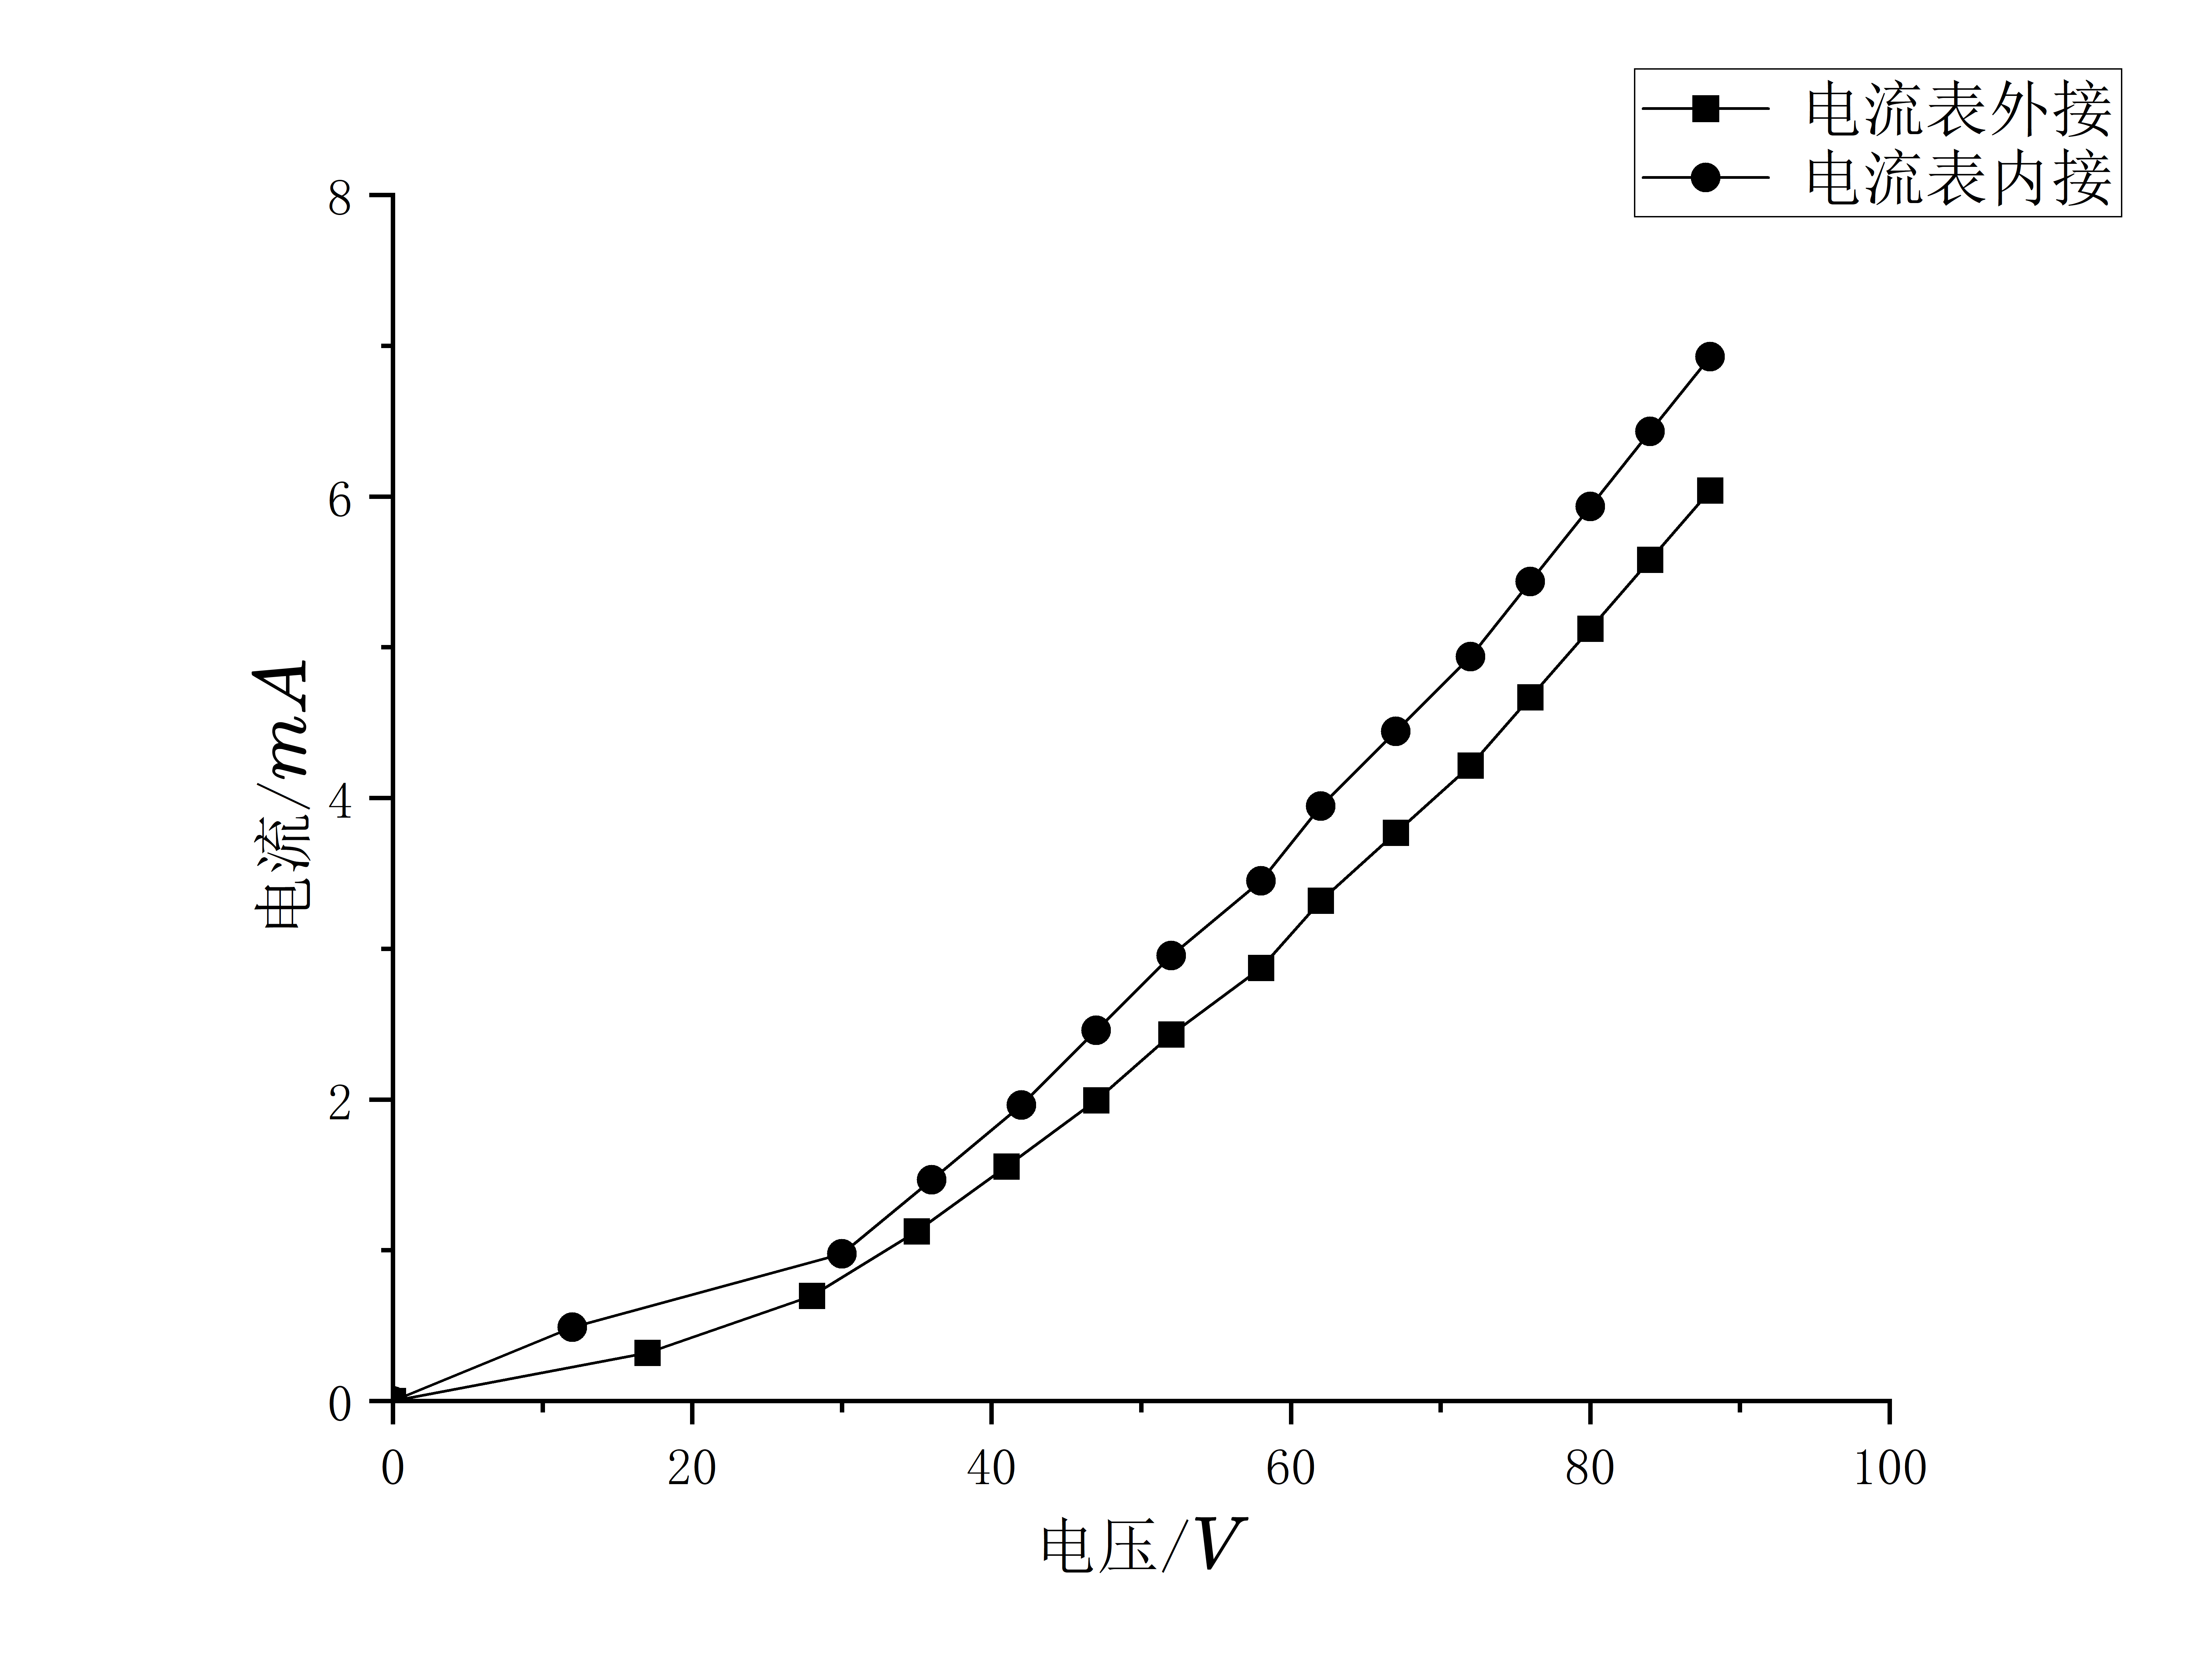
\includegraphics[width=10cm]{Figs/Graph1.png}
        \caption{钨丝小灯泡伏安特性曲线}
    \end{figure}

    由曲线可知:
    \begin{enumerate}
        \item V相同时,$I_{\text{内}}<I_{\text{外}}$。分析:由于$I_{\text{内}}=\dfrac{V}{R_{\text{灯}}+R_A},\;I_{\text{外}}=\dfrac{V}{R_{\text{灯}}}+\dfrac{V}{R_V}$。又有$R_{\text{灯}}^2+R_{\text{灯}}R_A+R_AR_V>0 \implies (R_{\text{灯}}+R_V)(R_{\text{灯}}+R_A)>R_{\text{灯}}R_V \implies \dfrac{1}{R_{\text{灯}}+R_A}<\dfrac{1}{R_{\text{灯}}}+\dfrac{1}{R_V} \implies \dfrac{V}{R_{\text{灯}}+R_A}<\dfrac{V}{R_{\text{灯}}}+\dfrac{V}{R_V} \implies I_{\text{内}}<I_{\text{外}}$。
        \item 内接法的伏安特性曲线整体位于外接曲线的左上方。内接法的误差来源:电流表分压,$\Delta V = I \cdot R_A$,误差随电流增大线性增加,导致小灯泡的等效电阻计算值偏大,$R_{\text{测}} = R_L + R_A$。外接法的误差来源:电压表分流,$\Delta I = \dfrac{V}{R_V}$,误差随电压增大线性增加,导致等效电阻计算值偏小,$R_{\text{测}} = \dfrac{R_L R_V}{R_L + R_V}$。
    \end{enumerate}
    \item 测量发光二极管的伏安特性曲线
    
    作绿色、蓝色发光二极管的正向伏安特性曲线(见图2)。
    \begin{figure}[H]
        \centering
        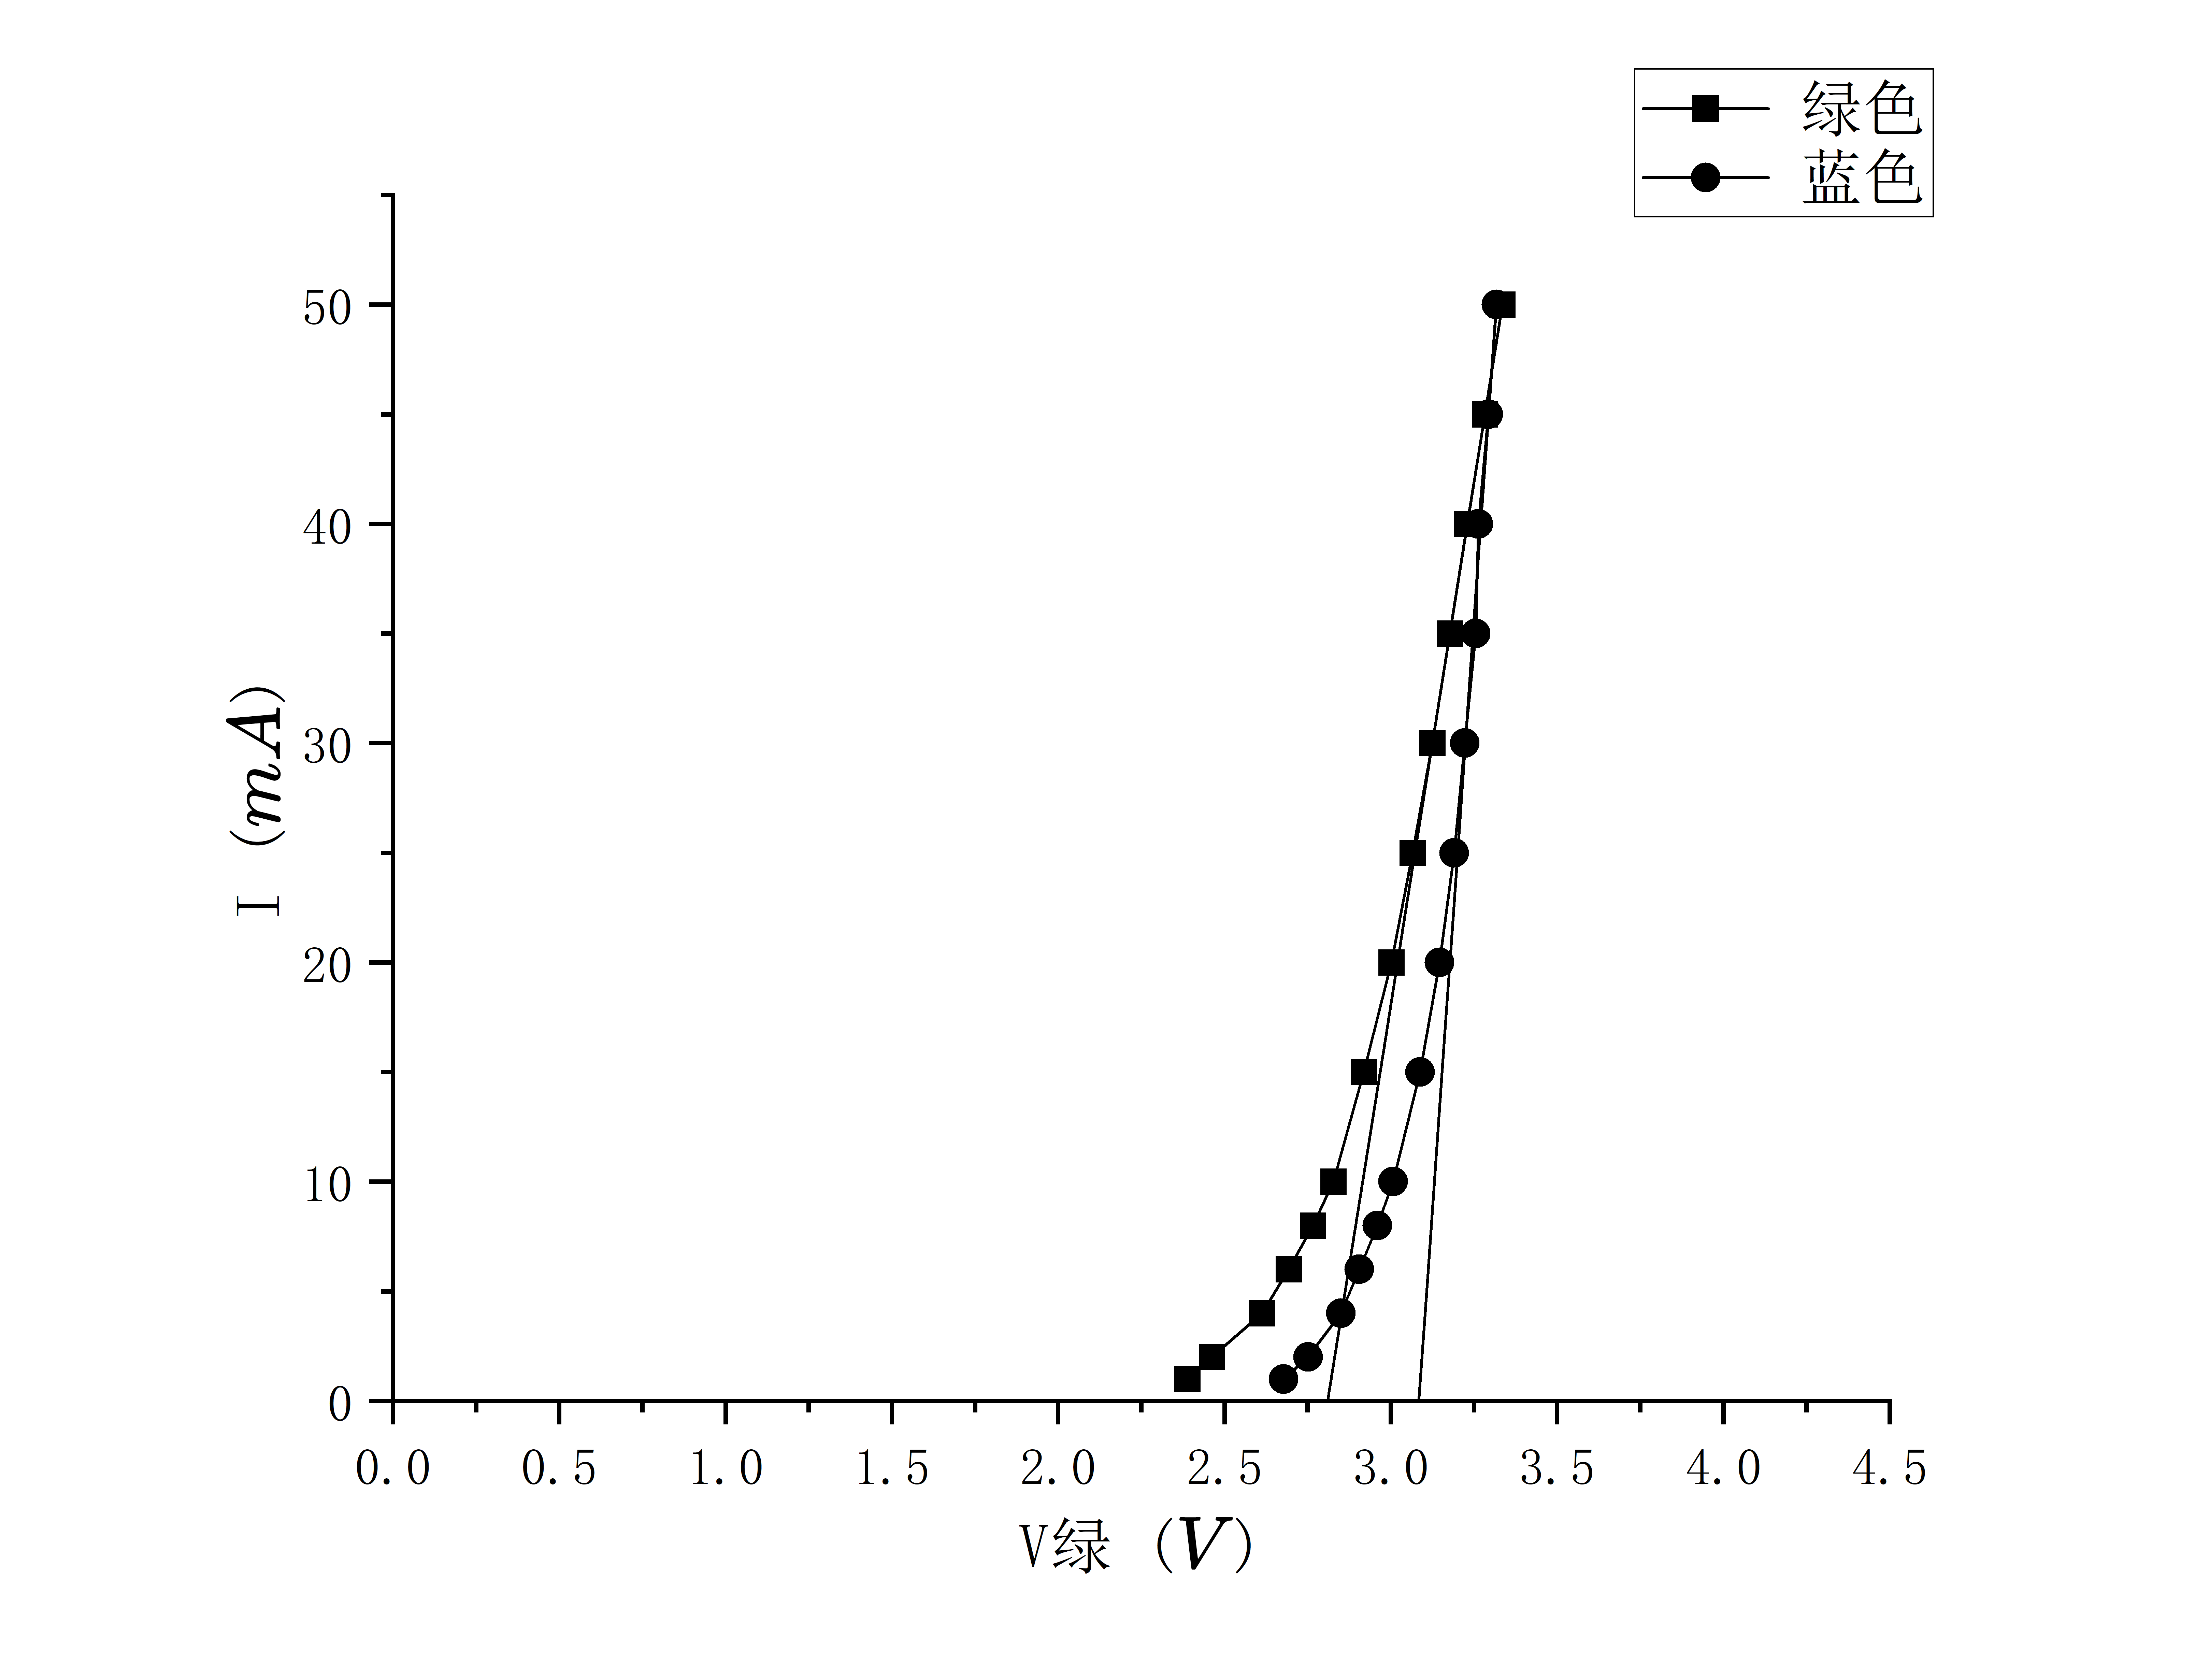
\includegraphics[width=15cm]{Figs/Graph2.png}
        \caption{发光二极管的伏安特性曲线}
    \end{figure}
    对两条曲线最后五组数据进行线性拟合,得到x轴截距,即两种发光二极管的阈值电压分别为$U_G=2.810\,V,\;U_B=3.085\,V$。由公式$eU_D=h\dfrac{c}{\lambda}$,即$\lambda=\dfrac{hc}{eU_D}$,得到两种发光二极管的波长分别为:
    $$
    \lambda_G=\dfrac{6.626\times10^{-34}\,J\cdot s \times 2.998\times10^8\,m\cdot s^{-1}}{1.602\times10^{-19}\,C\times2.810\,V}=441.3\,nm
    $$
    $$
    \lambda_B=\dfrac{6.626\times10^{-34}\,J\cdot s \times 2.998\times10^8\,m\cdot s^{-1}}{1.602\times10^{-19}\,C\times3.085\,V}=401.9\,nm
    $$
    
    \newpage

    \item 测量稳压二极管的伏安特性曲线
    
    作稳压二极管的正向与反向伏安特性曲线(见图3)。
    \begin{figure}[H]
        \centering
        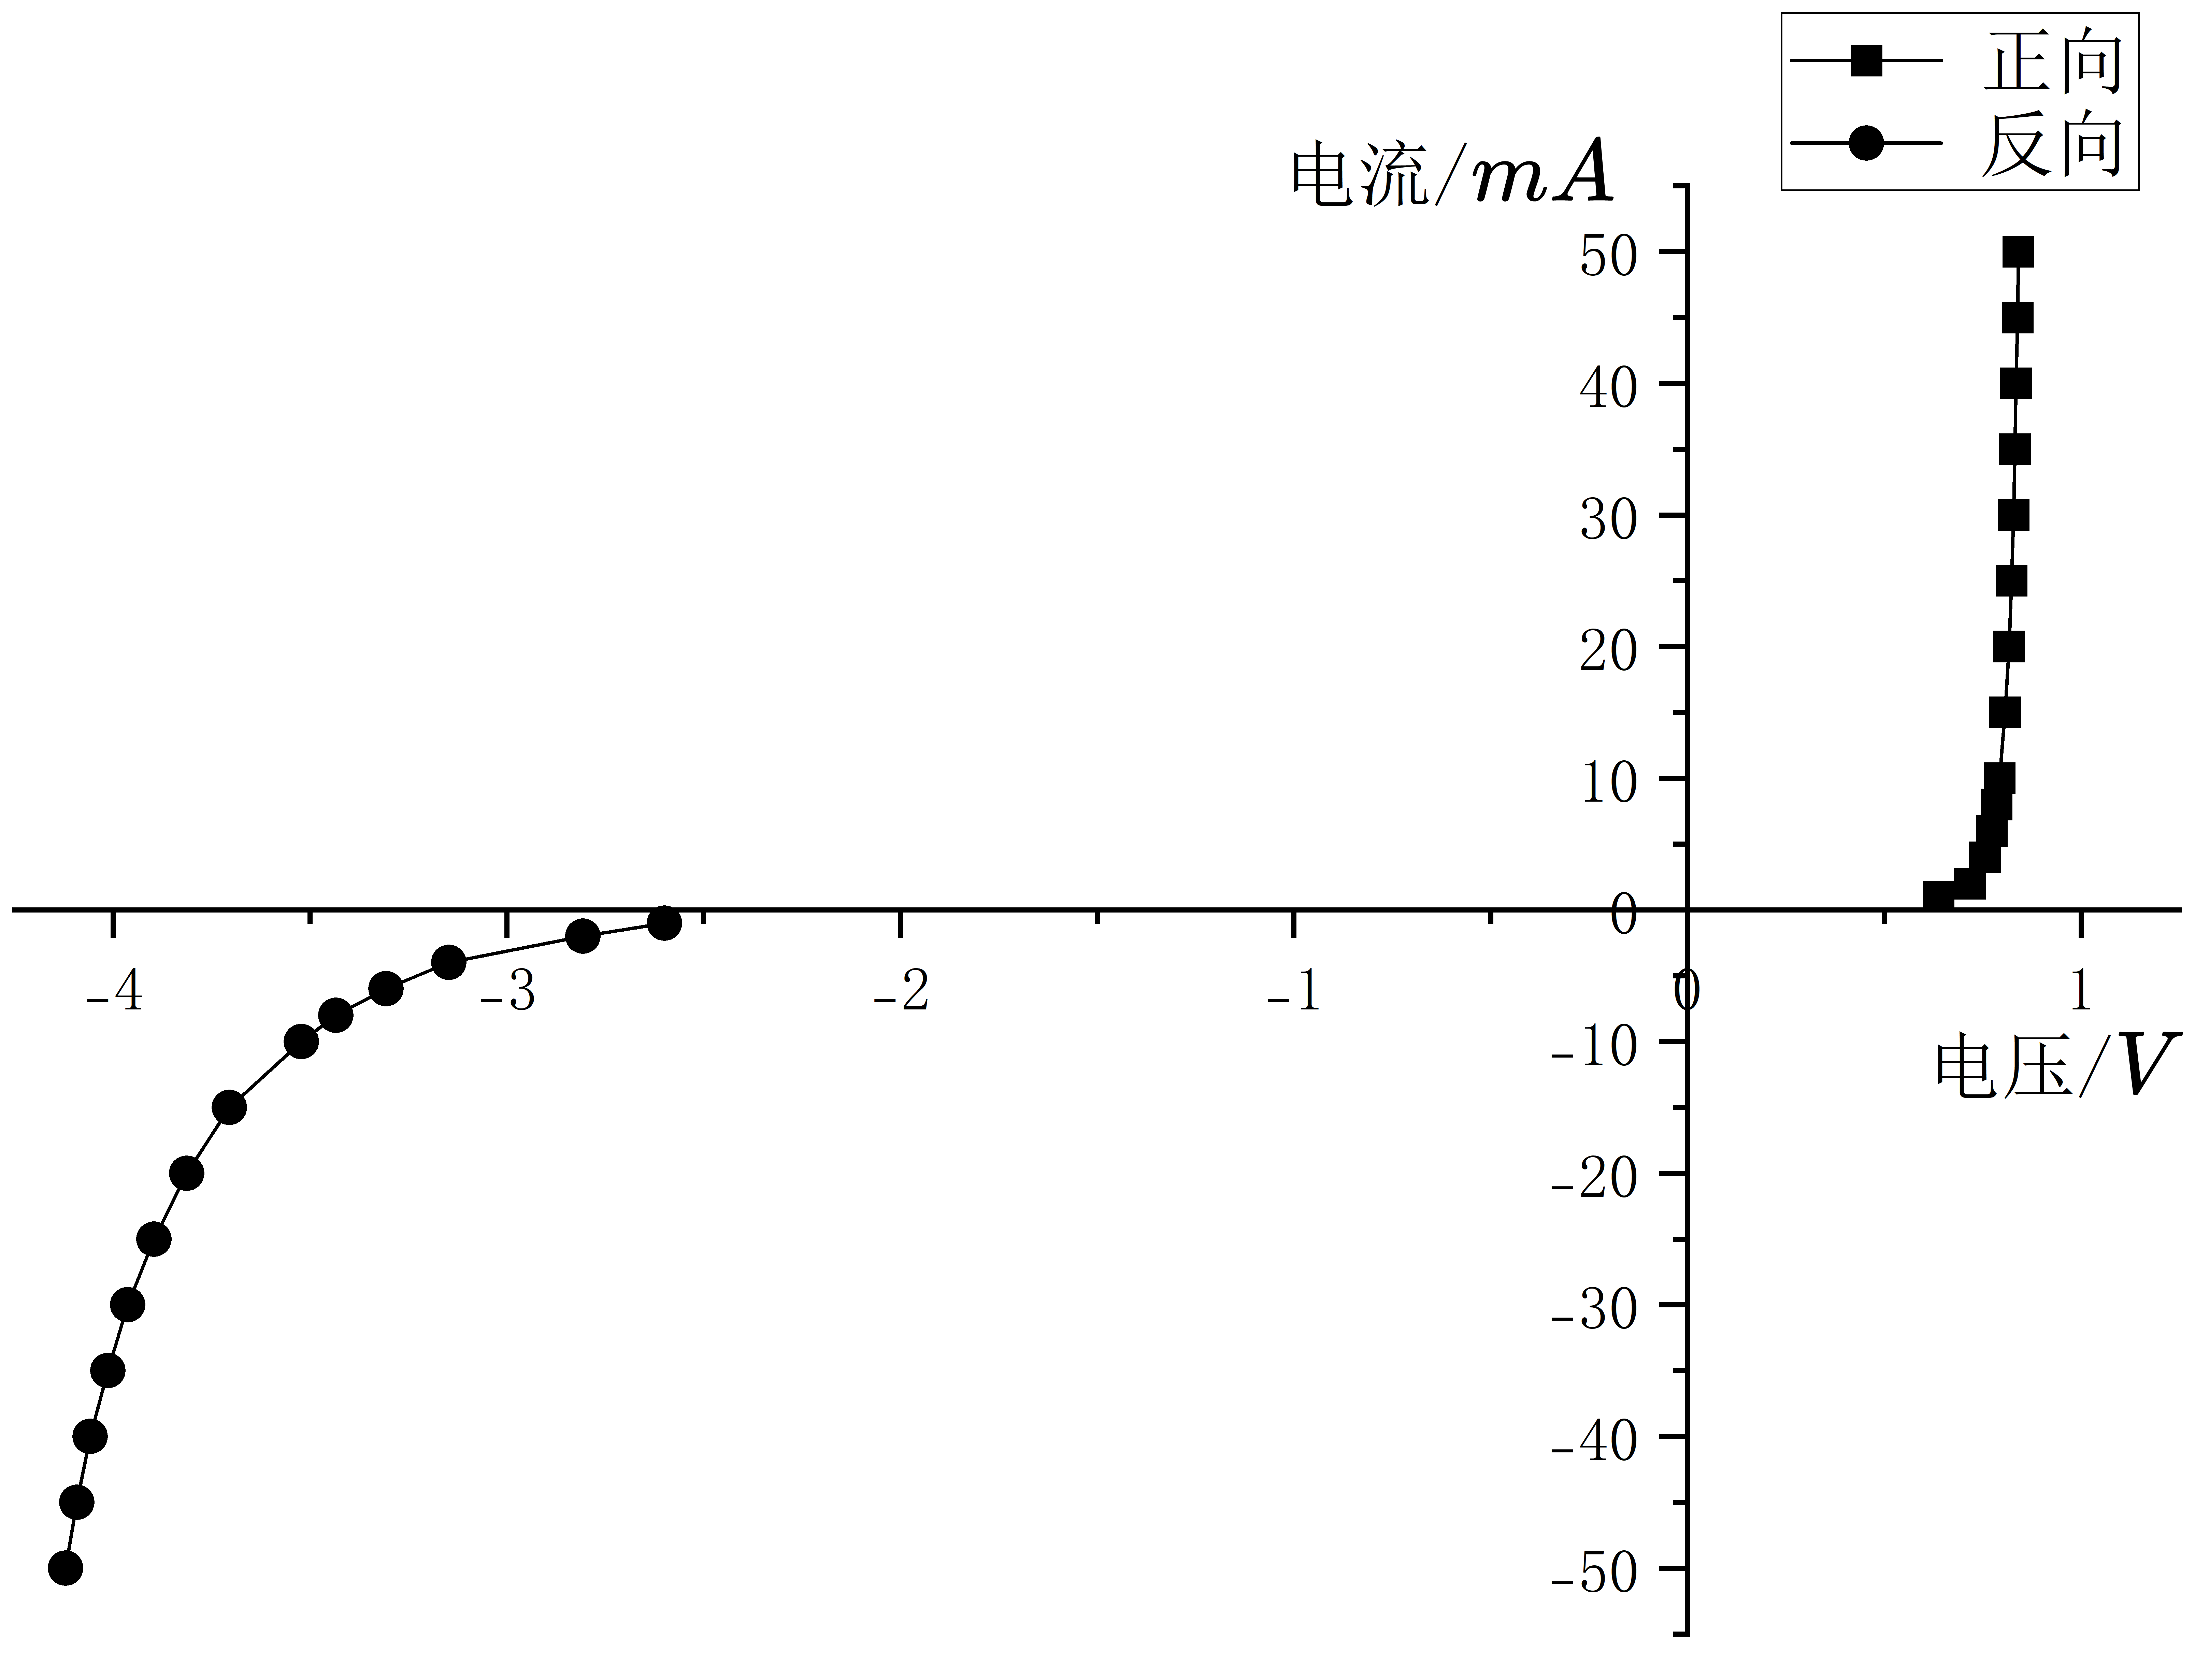
\includegraphics[width=12cm]{Figs/Graph3.png}
        \caption{稳压二极管的正向与反向伏安特性曲线}
    \end{figure}
\end{enumerate}

\section*{七、误差分析}

\begin{enumerate}
    \item 实验仪器精度不足;
    \item 导线有电阻;
    \item 发光二极管的光不是单色光,有杂光;
    \item 电流的热效应导致元件升温而电阻发生变化。
\end{enumerate}

\section*{八、思考题}

探讨\xcancel{三}两种颜色发光二极管伏安特性曲线的相似和不同之处?并做出合理的解释。
\\答:

相似之处:随着电压变大,曲线先缓慢上升,之后迅速爬升,且电压越大越接近于线性变化。

解释:正向电压较小时,二极管仍然处于截止状态,PN结的内建电场尚未被完全抵消,电子和空穴的扩散受到抑制,仅仅有少量电子流过形成小电流,电流随着电压变化较小,曲线平缓上升;电压大于开启电压后,二极管进入导通状态,亮度随电流迅速提升,伏安曲线斜率急剧增大,电流随电压成指数增长;电压继续增大,二极管一直处于导通状态,故电流随电阻呈线性增长。

不同之处:曲线的线性增长部分的延长线与x轴的交点不同,即阈值电压不同。

解释:制作不同的二极管所用的材料不同,故电子和空穴复合放出的能量不同。光的波长越短,意味着放出它所需的能量越高,从而它所对应颜色的发光二极管的阈值电压越大。

\section*{九、实验结论}

本次实验测量并绘制了钨丝小灯泡、绿色和蓝色发光二极管、稳压二极管正反向的伏安特性曲线。通过计算得到两种发光二极管发出光的波长分别为$\lambda_G=441.3\,nm,\;\lambda_B=401.9\,nm$。

\end{document}